\chapter{Implementation Details}\label{ch:implementation}

Host applications that support an embedded programming language, typically do so to increase end-user functionality.
For example, a web browser supports JavaScript to enable more interactive pages.
At the time developers introduce the ability to program their application, focus usually rests on extending existing functionality rather than any security implications raised by the ability to run user provided programs.
Side-effects of this prioritization can be seen in today's web ecosystem.

Because of an early and rapid rise in electronic commerce, web browsers now often manipulate, process, and relay sensitive information, including personal financial data.
A browser's support for JavaScript means that it remains possible for malicious code to steal the valuable information stored by the browser.
Recall that web browser architecture lacks (and sometimes impedes) important security properties (\autoref{ch:motivation}).
This state of affairs makes web sites a prime target for injected code attacks.
Consequently, the combination of historically poor security practices and the popularity of the web makes web browsers an ideal case study for retrofitting security into embedded language platforms.

Rather than fret over distinguishing between legitimate and malicious code (or buggy legitimate code), \JitFlow\ performs information tracking on all executed code.
This approach catches all malicious behavior defined by some security policy, forcing conformance even on trusted code.
\JitFlow\ adds information flow tracking infrastructure to JavaScriptCore.
The retrofitting of security into an established and mature VM occurs as four components:
(1) the labeling of the data types (\autoref{ch:label-propagaton}),
(2) the instrumentation of instructions for managing runtime data structures such as the control flow stack (\autoref{sec:control-flow-stack}) and program counter label,
(3) the implementation of JIT-complied versions of existing and new virtual machine instructions,
(4) and the introduction of memory layout modifications to stack frames that support caching of the \pclabel for fast retrieval and seamless switching between JIT-compiled code and the interpreter.

\newcommand{\popj}{\code{POPJ\_CFLABEL} }
\newcommand{\dup}{\code{DUP\_CFLABEL} }
\newcommand{\join}{\code{JOIN\_CFLABEL} }

\section{Control Flow Instructions}\label{sec:instructions}

The introduction of new instructions for the maintenance of the control flow stack permits a far easier JIT implementation of information flow.
These instructions serve to decouple the concerns of computation from information flow tracking.
Principally, they ensure that the control flow stack keeps alignment with the control flow structures of the program under execution.
Second, they cache the \pclabel in the stack frame, providing a fast and stable access point for all instructions, whether interpreted or JIT-compiled.
Finally, other virtual machines, such as SpiderMonkey, can adopt the same technique.

\subsection{The Necessity for New Instructions}

Initial implementing attempts to manipulate the control flow stack by modifying the functionality of existing instructions met with several obstacles which motivate the introduction of new instructions for maintaining the control flow stack.
These obstacles do not specifically affect only JavaScriptCore and SpiderMonkey, but originate from fall-through execution paths common to many languages.
The technique of extending the instruction set generalizes to other dynamically typed language runtimes.

When examining the instruction stream, the merge point of an \code{if-then-else} construct has no special distinguishing feature.
In some paths, a jump instruction targets the merge point, while in other paths execution arrives at the merge point via a fall-through.
Additionally, the instruction present at the merge point could be any of the existing instructions implemented by the VM.
Neither the instructions comprising the arrival path nor the instruction at the merge point itself can serve as a unique marker for identifying a merge point.
Because no runtime mechanism can identify the merge point based solely on a single path's sequence of executed instructions, \JitFlow\ instruments a \popj instruction at every merge point.
Not only does this instruction serve as a marker which locates the merge point, but it also performs the appropriate action on the control flow stack.

A more subtle difficulty occurs at the beginning of conditional branch and loop structures.
Primitive underlying compare-and-jump instructions serve to easily identify these these points.
Examination of the target offset of the jump instruction can even distinguish loops from a conditional branch.
Loops have a backward branch (negative offset) while all conditional branches point forward (positive offset).
Naively, we thought it might be possible to modify the behavior of the compare-and-jump instructions to push a label onto the control flow stack.
However, this approach produces an erroneous execution in loops: every iteration in a loop evaluates the conditional instruction, causing a push which breaks alignment of the control flow stack with respect to the execution history of program counter.
To ensure that only one label push occurs at entry into a loop, \JitFlow\ instruments a \dup instruction in the loop header.

Given the introduction of two instructions for manipulating the control flow stack, the \JitFlow\ framework can now reliably keep the 1-1 correspondence between labels on the stack and branches in control flow taken at runtime.
However, the evaluation of a conditional instruction also implies an upgrade to a new security context.
To satisfy this additional requirement, \JitFlow\ introduces the \join instruction, which upgrades the label on the top of the control flow stack using the label conditional controlling the branch.
Inserting this instruction between the computation of a conditional value and its use as a control flow branch allows both looping and branching constructs to compute the correct security context.

Treatment of return statements requires further analysis
\JitFlow\ must take care to align the control flow stack height in the event that a return occurs inside a nested code block.
A translation of the return into a three step process accomplishes this task.
First, label the return value using the current top of the control flow stack (i.e. the \pclabel) and cache the value in the stack frame.
Second, instrument a \popj to restore the control flow stack height.
Third, return the properly labeled value and tear-down the function.
In a register machine, such as JavaScriptCore, the return instruction implementation can perform all three steps, by extending the return instruction opcode with an immediate value representing the control flow stack depth.

\subsection{Control Flow Stack Instruction Details}

The JavaScript VM first compiles each script into an instruction stream before beginning interpretation.
\JitFlow\ modifies the parser to produce an instruction stream that differs only by the addition of control flow instructions which track and record control flow paths executed at runtime.
During parsing, a static analysis provides the instruction emitter knowledge of nesting levels and control flow depth.
This information determines the values of parameters which control the number of pushes, pops, or joins carried out by the control flow stack at runtime.
To ensure that the parser performs instrumentation correctly, an abstract interpreter verifies, over all possible paths, a consistent control flow depth for each instruction in the stream.
Using the instrumented instructions at runtime, \JitFlow\ maintains a 1-1 correspondence between the number of labels on the control flow stack and the number of control flow branches taken during program execution.

\lstset{caption={Hypothetical information leak of secret variable \code{pin}, using an active implicit information flow.},
        label=list:steal-pin}
\begin{jscode}
function stealpin() {
  for (var i=0; i < 100000; ++i) {
    if (i == pin) break;
  }
  return i;
}
\end{jscode}

The code sample in \autoref{list:steal-pin} contains control flow structures, such as a \code{for}-loop, \code{break} statement, and \code{return} statement which allows us to examine the placement of the control flow stack instructions in greater detail.
An attacker manages to inject the \code{steal\_pin} function, manufactured so that, at the end of execution, the local variable \code{i} contains the same value as the secret variable \code{pin}.

Despite the fact that other, more direct mechanisms can achieve this relationship, the example highlights lesser used control flow constructs, such as the \code{break} statement, and the impact these constructs have on maintaining the control flow stack height.

\begin{figure}[h]
\begin{python}
code = r'''
function stealpin() {
  for (var i=0; i < 100000; ++i) {
    if (i == pin) break;
  }
  return i;
}

print(debug(stealpin))
'''
import sys
sys.path.append('..')

import jsc
j = jsc.jsc(code)
j.run()

import bytecodeformatter
bytecodeformatter.tikz_picture(j.instructions())
\end{python}
  \caption{\JitFlow\ instruction stream representing the code snippet in \autoref{list:steal-pin}.}
  \label{fig:steal-pin-bytecode}
\end{figure}

\subsubsection{\dup}

\begin{samepage}
\begin{description}
  \item[Operation] \hfill \\
    Duplicate the top label of the control flow stack.
  \item[Control Flow Stack] \hfill \\
    \ldots, label, $\Rightarrow$ \ldots, label, label
\end{description}
\end{samepage}

The \dup instruction duplicates the top of the control flow stack.
\JitFlow\ places this instruction before every control flow branch.
In many cases, this instruction pairs with a \join instruction which then upgrades the top of the control flow stack after evaluating the boolean condition of the branch.
In all cases, a corresponding \popj instruction later delineates the end of the secure region.

As shown in \autoref{fig:steal-pin-bytecode}, the loop header occurs after the loop body.
A \dup instruction at offset~\code{01} occurs prior to evaluation of the loop initialization code.
The presence of this instruction prepares the control flow stack for the secure region delineated by the loop.
A corresponding \popj instruction at offset~\code{41} occurs on a fallthrough out of the loop restoring the control flow stack height.
A second secure region, delineated by the \code{if}-statement inside the loop, can be found with a \dup instruction at offset~\code{07} and its corresponding \popj instruction offset~\code{27}.

% Was true in Firefox, but not true in FlowCore
% As can be seen at offset , our system also inserts an additional \texttt{DUP\_CFLABEL} instruction at the beginning of every function.
% This instruction provides each function with an additional label on the control flow stack that clearly delineates the function boundary, and provides an explicitly labeled operating context for all calculations performed within the function body.
% Before the function returns, a corresponding \texttt{POP\_CFLABEL} instruction (line~\texttt{56}) restores the state of the control flow stack.

\subsubsection{\join}\label{sec:join-cflabel}

\begin{samepage}
\begin{description}
\item[Operation] \hfill \\
 Upgrade the label at the top of the control flow stack by performing a lattice join with the label of the topmost value of the operand stack.
\item[Control Flow Stack] \hfill \\
 \ldots, label\subscript{a} $\Rightarrow$ \ldots, label\subscript{a} $\sqcup$ label\subscript{b}
\end{description}
\end{samepage}

A \join instruction supports upgrading the label of the program counter by joining the top of the control flow stack with the label of a given value.

This instruction proves necessary for supporting loop structures that continue or exit based on a boolean condition evaluated at runtime.
Because the condition depends on a runtime evaluation, each iteration through the loop may carry a different security label.

\JitFlow\ retains the successive joins of all iterations as it progresses through the loop.
A side effect of this design means that the evaluation of last iteration in a \code{for}-\code{in} loop over an array might occur under a higher security label than the first iteration.
For example, this situation occurs when the array consists of heterogeneously labeled fields.
Although finding ways to prevent such joins remains worthy of further research, we speculate that doing so safely would require analysis proving non-interference between successive iterations.

In the running example (\autoref{fig:steal-pin-bytecode}), the \join instruction at offset~\code{36} takes care of upgrading the current execution context at each iteration of the \texttt{for}-loop.
For the simple loop given in the example, upgrading the top of the control flow stack proves wasteful, because every iteration occurs under the same security context.
\JitFlow\ does not currently perform a more extensive analysis that would help identify this situation and optimize the join away.
Inside the \texttt{for}-loop, a \join instruction at offset~\code{17} upgrades the program counter based on the condition of the \texttt{if}-statement.

Note that incrementing the loop index variable (offset~\texttt{30}) occurs outside the context of the inner \texttt{if}-statement.
Even though we, as programmers, can see that the \code{break} statement enforces a dependence of the loop index variable on the secret variable \texttt{pin}.
\JitFlow\ therefore contains another instruction which enables tracking this dependence over the \code{break} statement.

\subsubsection{\popj}

\begin{samepage}
\begin{description}
\item[Operation] \hfill \\
 Pop $p$ labels from the top of the control flow stack, then perform a lattice join on each of the next $j$ labels on the control flow stack with the previous topmost label.
\item[Control Flow Stack] \hfill \\
  \ldots, label\subscript{i}, label\subscript{i+1} \ldots, label\subscript{i+j}, label\subscript{i+j+1}, \ldots, label\subscript{i+j+p}\\
 $\Rightarrow$
 \ldots, label\subscript{i}, label\subscript{i+1} $\sqcup$ label\subscript{i+j+p}, \ldots, label\subscript{i+j} $\sqcup$ label\subscript{i+j+p}
\end{description}
\end{samepage}

The \popj instruction carries two parameters: $p$, which specifies how many levels of control flow to pop, and $j$, which specifies how many further control flow levels that should be upgraded.
When the interpreter encounters a \popj instruction, it first saves the current top of the control flow stack, then it pops $p$ levels, and finally in-place joins $j$ more levels using the previously saved top.

In its primary role, the \popj instruction marks the position of every control flow merge and serves to pop a label from the control flow stack.
In the event that many control flow paths merge at the same point, the \popj instruction carries a parameter $p$, which indicates how may merges coincide.
For example, this situation may occur during an early return from within a nested loop.

In the example shown in \autoref{list:steal-pin}, both the \code{for}-loop and the \code{if}-statement each require only a single label to be popped from the control flow stack.
The \popj instruction at offset~\code{41} marks the end of the \code{for}-loop and the \popj instruction at offset~\code{27} marks the merge point of the \code{if}-statement.
Both of these occurrences pop a single secure lexical region from the current control flow stack, restoring it to the height it had prior to entry of the control structure, according to the rules in \autoref{sec:control-flow-stack}.

The presence of the second argument, $j$, which gives a depth of how many further control flow scopes should be upgraded after popping, enables \JitFlow\ to correctly handle \code{break} and \code{continue} statements.
These statements cause a divergence in control flow from within a nested scope out to a lexical outer scope.
As shown in the example in \autoref{list:steal-pin}, the \code{break} statement enforces a equality of the secret variable, \code{pin} and the loop index variable, \code{i}.
Having established this relationship, the malicious code can pilfer information via the variable $i$ because JavaScript semantics cause loop index variables declared with the \code{var} keyword to be promoted to function-level scope.
As a result, \JitFlow\ conservatively upgrades the entire function context via the joining operation incorporated into the \popj instruction.

When the nested \code{break} statement executes (\autoref{list:steal-pin}), the control flow stack contains three labels: one for the function, one for the \code{for}-loop, and one for the \code{if}-statement.
As shown in \autoref{fig:steal-pin-bytecode}, prior to exiting the loop due to the \code{break} statement, a \popj instruction at offset~\code{22} adjusts the control flow stack by popping the label of the \code{if}-statement (parameter $p$=1) and upgrades both the \code{for} loop and the current function scope (parameter $j$=2).
The \code{for}-loop then exits and the interpreter pops one label from the control stack (offset \code{41}), leaving only the label for the function scope left on the stack.

As noted previously, the inner \code{if}-statement does not directly influence the label attached to the loop index variable,~\code{i}.
Without upgrading this label, the \code{return} at line~\code{5} of \autoref{list:steal-pin} leaks the information of the secret variable \code{pin}.
However, the \popj instruction at offset~\code{22} upgrades the entire function context.
So any operations taking place after the occurrence of the \code{break} statement execute under a label at least as secure as the scope in which the \code{break} resides.
In particular, the \code{ret} instruction at offset~\code{44} executes under the upgraded label.
\JitFlow\ modifies the \code{ret} instruction to upgrade the label of the returned value by joining it with the label of the current execution context.
This action tracks the information flow demonstrated by \autoref{list:steal-pin}.

\section{Tracking Information Flow in the JIT}

Whether an interpreter or JIT-compiled code performs information flow tracking, the implementation requires supporting data structures and other modifications to the runtime VM.
This section presents the lower-level implementation which allows the JIT compiler to perform this tracking at substantially improved speeds.
Each modification focuses on increasing the performance of the tracking engine to support runtime compilation of code in \JitFlow.

\subsection{Label Encoding}

When implementing information flow logic in the JIT compiler, native functions impose an additional design constraint.
JavaScriptCore's JIT compiler interpreter require a unified representation that supports passing \jsvalues\ between native functions (implemented in C++) and JIT-compiled JavaScript functions.
The \term{inline label} representation results in high performance, so \JitFlow\ modifies the \JSValue\ representation as detailed in \autoref{sec:jitflow-labelencoding}.
The label resides in bits 32--47 of integers, pointers, and immediates, while doubles remain implicitly labeled with the highest available label in the lattice.

\subsection{Tracking Data Flow}

\JitFlow\ modifies JIT compiler in JavaScriptCore to track information flow in all binary operations:  \code{add}, \code{sub}, \code{mul}, \code{div}, \code{mod}, \code{lshift}, \code{rshift}, \code{urshift}, \code{bitand}, \code{bitor}, and \code{bitxor}.
Because JavaScript semantics allow for ad-hoc polymorphism, i.e., using the arithmetic add operator to perform both, numeric addition and string concatenation, the \code{add} operation supports multiple data types.

\lstset{
  caption={Label propagation for the numeric \code{add} instruction, with left and right integer operands in registers \code{RAX} and \code{RBX} respectively.
  Registers \code{R11} and \code{R12} serve as scratch registers for computing the labels encoded in bits 32--47.},
  label={list:jitflow-propagation},
}
\begin{asmcode}
// to join the labels of RAX and RBX
// move the first value (including label) into scratch register
MOV R11, RAX
// then bitwise-or first value (including label) with second value
OR  R11, RBX

// to join the cached top of the label stack
// first load the cached top-label of the pc-stack into scratch register
MOV R12, [RSP+60h]
// then bitwise-or the top-label of the pc-stack with operand labels
OR  R11, R12

// mask out value bits, so only label bits remain in R11
// first load the label-bit-mask into scratch register
MOV R12, 0FFFF00000000h
// then bitwise-and label-bit-mask with accumulated label
AND R11, R12

// perform the 32-bit add operation
ADD EBX, EAX
// bitwise-or the result with the joined label
OR  RBX, R11
\end{asmcode}

\autoref{list:jitflow-propagation} illustrates how the JIT compiler performs label propagation, by providing a simplified portion of the assembly code emitted by the JIT compiler for integer addition.
The binary operation has been split into three parts to give a precise description of each computation step:

\subsubsection{Joining Operand Labels}

As illustrated, \code{RAX} holds the left operand and \code{RBX} holds the right operand.
Registers \code{R11} and \code{R12} serve as scratch registers for the label propagation calculation.
Because the calculation of the addition and the propagation of the label must be kept separate, the code first copies the value of the left operand (including its label) into register \code{R11} (\codeline{2}).
Without masking out the label, \JitFlow\ joins in the value (and label of) the right operand using a bitwise-or (\codeline{3}).
At this point, \code{R11} contains the join of the labels of both operands together with the bitwise-or of the values.

The label on the result of the addition must also include the label from the current context.
Because the top of the control flow stack provides the security context to every binary operation, \JitFlow\ caches it in the \code{JITStackFrame} (\autoref{sec:jitcontrolflow}).
Line~6 retrieves the label from the cache into register \code{R12}.
The VM joins in this context label using another bitwise or, accumulating the result in register \code{R11} (\codeline{7}).

Register \code{R11} now contains the final label that will be attached to the result of the addition.
However, some non-label bits within the register remain non-zero as a result of using the operand values directly.
Unfortunately, x86\_64 architecture does not support 64~bit immediate operands for the bitwise and operator, so masking out the value bits requires two steps.
First, \JitFlow\ loads a label mask, which has only bits 32--47 set to one, into register \code{R12} (\codeline{10}).
Next, the mask and accumulated label undergo bitwise and, leaving only the label's bits active in register \code{R11} (\codeline{11}).

\subsubsection{Performing the Operation}

After calculating the label, the \JitFlow\ performs the addition of the two operands (\codeline{13}) with a 32~bit add instruction.
For simplification, the example elides an overflow check that occurs immediately after the addition.
In practice, this check makes use of the overflow and carry flags and transfers control to a slow path that coerces the input integers into doubles.

\subsubsection{Assigning the Accumulated Label}

Assuming the addition finished without overflow, the last step combines the accumulated label and the computed result value.
\JitFlow\ does not have to mask out any active bits within the label field of the result value before the label assignment because of two observations.
First, the addition operation operates on 32~bits and only affects the value portion, not the label field.
Second, any active label bits in the result come from an input operand and form a strict subset of the active bits in the accumulated label (register~\code{R11}).
Together, these properties allow \JitFlow\ to use bitwise-or to apply a label to the result value in register \code{RBX} (\codeline{15}).

\subsection{Tracking Control Flow}

%\JitFlow\ inherits the same technical difficulties regarding the semantics of the JavaScript language that \FlowCore\ addressed.
%The lack of static typing pushes \JitFlow\ to use the same control flow stack for propagating the influence that a branch in control flow has over operation within the branch.
%\JitFlow\ uses \FlowCore's parser to emit the \dup, \join, and \popj instructions that assist in tracking control-flow joins and branches as the program executes.
At parse-time, \JitFlow\ instruments the control-flow stack instructions into the instruction stream and annotates the function with a maximum control-flow stack depth.
When the function executes, \JitFlow\ pre-allocates space for the control flow stack as part of setting up stack frame.

As explained in \autoref{sec:instructions}, JavaScript complicates the context tracking issue by supporting labeled \code{break} and \code{continue} statements that cause early exit from arbitrarily nested inner loops.
When a program performs one of these scope-jumping actions, all further operations carried out within the function become tagged with the label under which the break or continue occurred.
\JitFlow\ accomplishes this tracking with a stack of labels that follow the program counter and issuance of a \popj instruction that upgrades the function's entire control flow stack.
To briefly illustrate this process, \autoref{list:jitflow-stealpin-bytecodes} contains the instruction sequence for the \code{stealpin} function shown in \autoref{list:steal-pin}.

\lstset{
}
\begin{figure}[h]
\begin{python}
code = r'''
function stealpin(secret) {
  for (var i=0; i < 10000; i++) {
    if (i == secret)
      break;
  }
  return i;
}

print(debug(stealpin))
'''
import sys
sys.path.append('..')

import jsc
j = jsc.jsc(code)
j.run()

import bytecodeformatter
bytecodeformatter.tikz_picture(j.instructions())
\end{python}
  \caption{Instruction sequence of the \code{stealpin} function in \autoref{list:steal-pin}.}
  \label{list:jitflow-stealpin-bytecodes}
\end{figure}

Immediately after entry, the \code{stealpin} function contains a loop that begins with the \dup\ instruction (\bcodeline{01}) that pushes a new security scope for the loop body.
JavaScriptCore places the condition at the end of the loop body, so the \join\ instruction that upgrades the security scope corresponding to the loop belongs on \bcodeline{31}.
After evaluating the condition, the loop body begins at \bcodeline{07}.

The loop body consists of an \code{if}-statement that acts as a nested security scope.
This scope begins with a \dup\ instruction (\bcodeline{07}) and gets upgraded (\bcodeline{12}) after evaluation of the conditional (\bcodeline{08}).
Should the condition fail, control flow branches to \bcodeline{22} which pops a label off the control flow stack indicating the end of the \code{if}-statement.
When the condition succeeds, the body of the \code{if} executes the \code{break} statement.
A \popj\ instruction (\bcodeline{17}) precedes the jump (\bcodeline{20}) that directs control flow out of the loop.
This instruction causes \JitFlow\ to pop the scope corresponding to the \code{if}-statement (argument \code{pop:1}) and to upgrade two levels below it (argument \code{join:2}), corresponding to the loop body and the function itself.

Regardless of the path through the loop, finishing with the normal exit or by following the \code{break} statement, the loop ends with a \popj\ instruction (\bcodeline{36}) that restores the control flow stack to the level it had before loop entry.

\subsection{Optimizing Control Flow Tracking in the JIT}\label{sec:jitcontrolflow}

The steps taken to increase JIT compiler performance for tracking control flow involved successive refinement.
For example, JavaScriptCore's JIT compiler does not fully implement all of the bytecode instructions and often calls back into the interpreter to handle slow paths.
At one stage during development, the \JitFlow\ compiler implemented our the new control-flow instructions (\autoref{sec:instructions}) through a callback to C++.
This stage of implementation naturally had a higher performance overhead than the final product.

\JitFlow\ uses three techniques to enable fast tracking of control-flow influence:
\begin{enumerate}

\item \textit{It pre-allocates memory for the control-flow stack}, just as an unmodified JavaScriptCore pre-allocates an array for the call-frame stack.
Rather than allocating a small control-flow stack for each function frame, which negatively impacts runtime performance, each JavaScript function call now reserves space on a global control-flow stack for the number of labels that it requires for worst-case nesting depth.
Reservation of this space amounts to incrementing a stack pointer in the pre-allocated array, analogous to bump allocation in memory management.

\item \textit{It caches the top label of the control-flow stack.}
Ordinarily, the information-flow tracking VM finds the label of the current execution context by following a chain of references that starts at the \code{CallFrame} pointer in the current \code{StackFrame}, traverses through the control-flow stack pointer in the current \code{CallFrame} and finally ends at an offset from the base of the current control-flow stack.
Because all data-flow operations also join in the current program counter label, \JitFlow\ caches the top of the control-flow stack in the \code{StackFrame} data structure so that it remains accessible through a fixed offset from the \code{StackFrame}.
\autoref{fig:jitflow-stackframe} shows both the chain of references and the cache location.

\begin{figure}[ht]
  \centerline{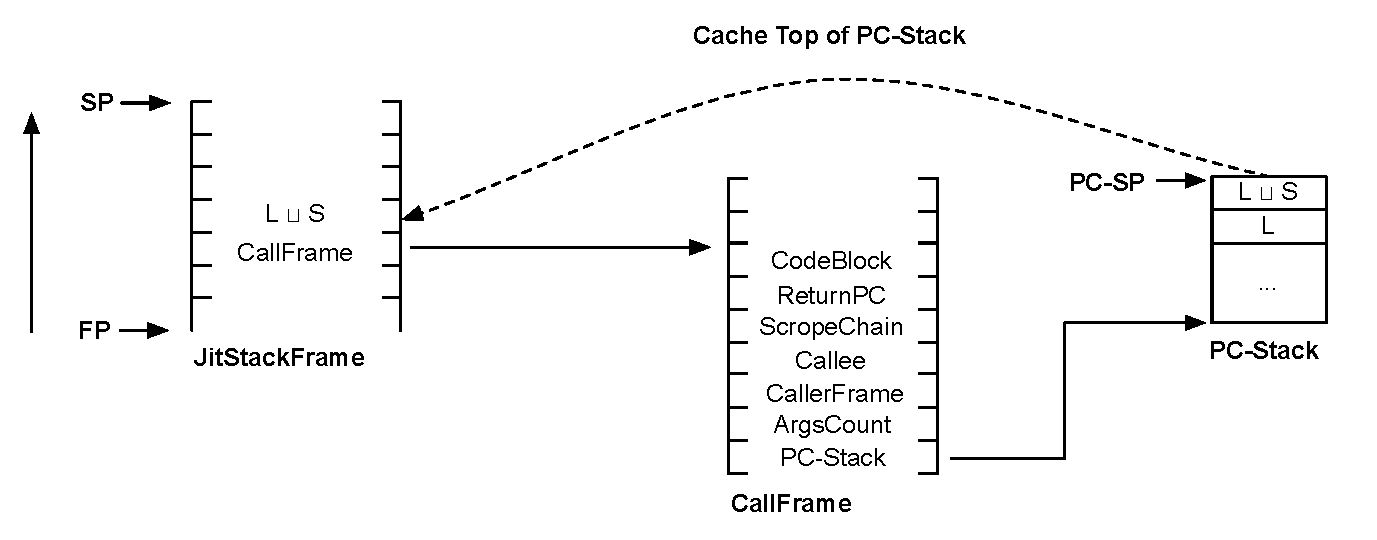
\includegraphics[width=\linewidth,keepaspectratio=true]{graphics/stackframe.pdf}}
  \caption{Interaction of native \code{JITStackFrame}, \code{CallFrame}, and Control-flow stack.}
  \label{fig:jitflow-stackframe}
\end{figure}

\JitFlow\ updates this cache every time the top label of the control-flow stack changes.
This update occurs at control-flow branches and joins and happens less frequently than the data-flow operations that access the top label.

Additionally, using such a caching mechanism allows \JitFlow\ to avoid expensive updates on top of the control-flow stack if the label of the predicate and the cached label remain identical.
As previously mentioned, the instruction \join\ upgrades the top of the control-flow stack by joining it with the label of the predicate value.
To avoid such unnecessary updates, \JitFlow\ emits compiled code that first checks the equality of the cached label in the \code{JITStackFrame} and the label of the predicate.
If so, the runtime system skips the expensive task of following the pointers to update the top of the control-flow stack because it already holds the correct label.

\item \textit{It implements the instructions that maintain the control-flow stack directly in assembly.}
%\JitFlow\ takes as input the same instruction stream as the \JitFlow\ interpreter.
When the JIT compiler encounters one of the control-flow stack manipulation instructions (\autoref{sec:instructions}) it emits assembly code that performs the operation.
Not only does this code access the control-flow stack through the appropriate reference path shown in \autoref{fig:jitflow-stackframe}, but it also updates the cached top label when necessary.
Cache updates only occur in the \join\ and \popj\ instructions, because the \dup\ instruction modifies stack height but does not change the label on top.

Implementing the instructions that maintain the control-flow stack (\dup, \join, and \popj) in assembly code avoids expensive callbacks into C++ at runtime, allowing \JitFlow\ to increase speed by not having to (i) save and restore registers when calling into C++ and (ii) perform the expensive trampoline jump to find the function entry point in C++.

\end{enumerate}

Only by implementing all of these techniques could  \JitFlow\ achieve the low-overhead performance measured in \autoref{sec:jitflow-evaluation}

